\documentclass[main.tex]{subfiles}

\section{ESDIRK23}

\subsection{Implementation with fixed step size}
Following the hint given at the lecture, the ESDIRK code from lecture files was used as a base to implement the fixed step size ESDIRK23. Given source is inspired by Tobias Ritschel's work on Numerical Methods For Solution of Differential Equations, however we aren't concerned about the modified version which uses function $g$ as slightly modified initial value problem. Also fixed step size obviously doesn't require step size control so that part is removed.

Matlab code for this implementation is in the appendix.

\subsection{Testing on Van der Pol problem and comparison with our designed ERK}
%Test your implementation on the Van der Pol equation with µ = 3 and
%µ = 100. Compare the solution and the number of function evaluations
%with your own Explicit Runge-Kutta method.
The problem for the given $\mu$ of 100 is stiff as can be seen on figure \ref{fig:ex5comparison} (second row) since the function values change a lot in very small timespan (mix of red and blue points). The step size was set to $0.001$ and absolute and relative tolerances to $10^{-6}$. Next we want to compare the previously designed ERK with ESDIRK23 in number of function evaluation in the method. For $\mu = 3$ the problem isn't stiff and ESDIRK23 has more function evaluations than ERK (60942 vs 60000), however when $\mu = 100$, ESDIRK23 computes 403695 evaluations versus 600000 of ERK resulting in almost 33\% decrease and making ESDIRK23 better candidate for stiff problems.
\begin{figure}[H]
    \centering
    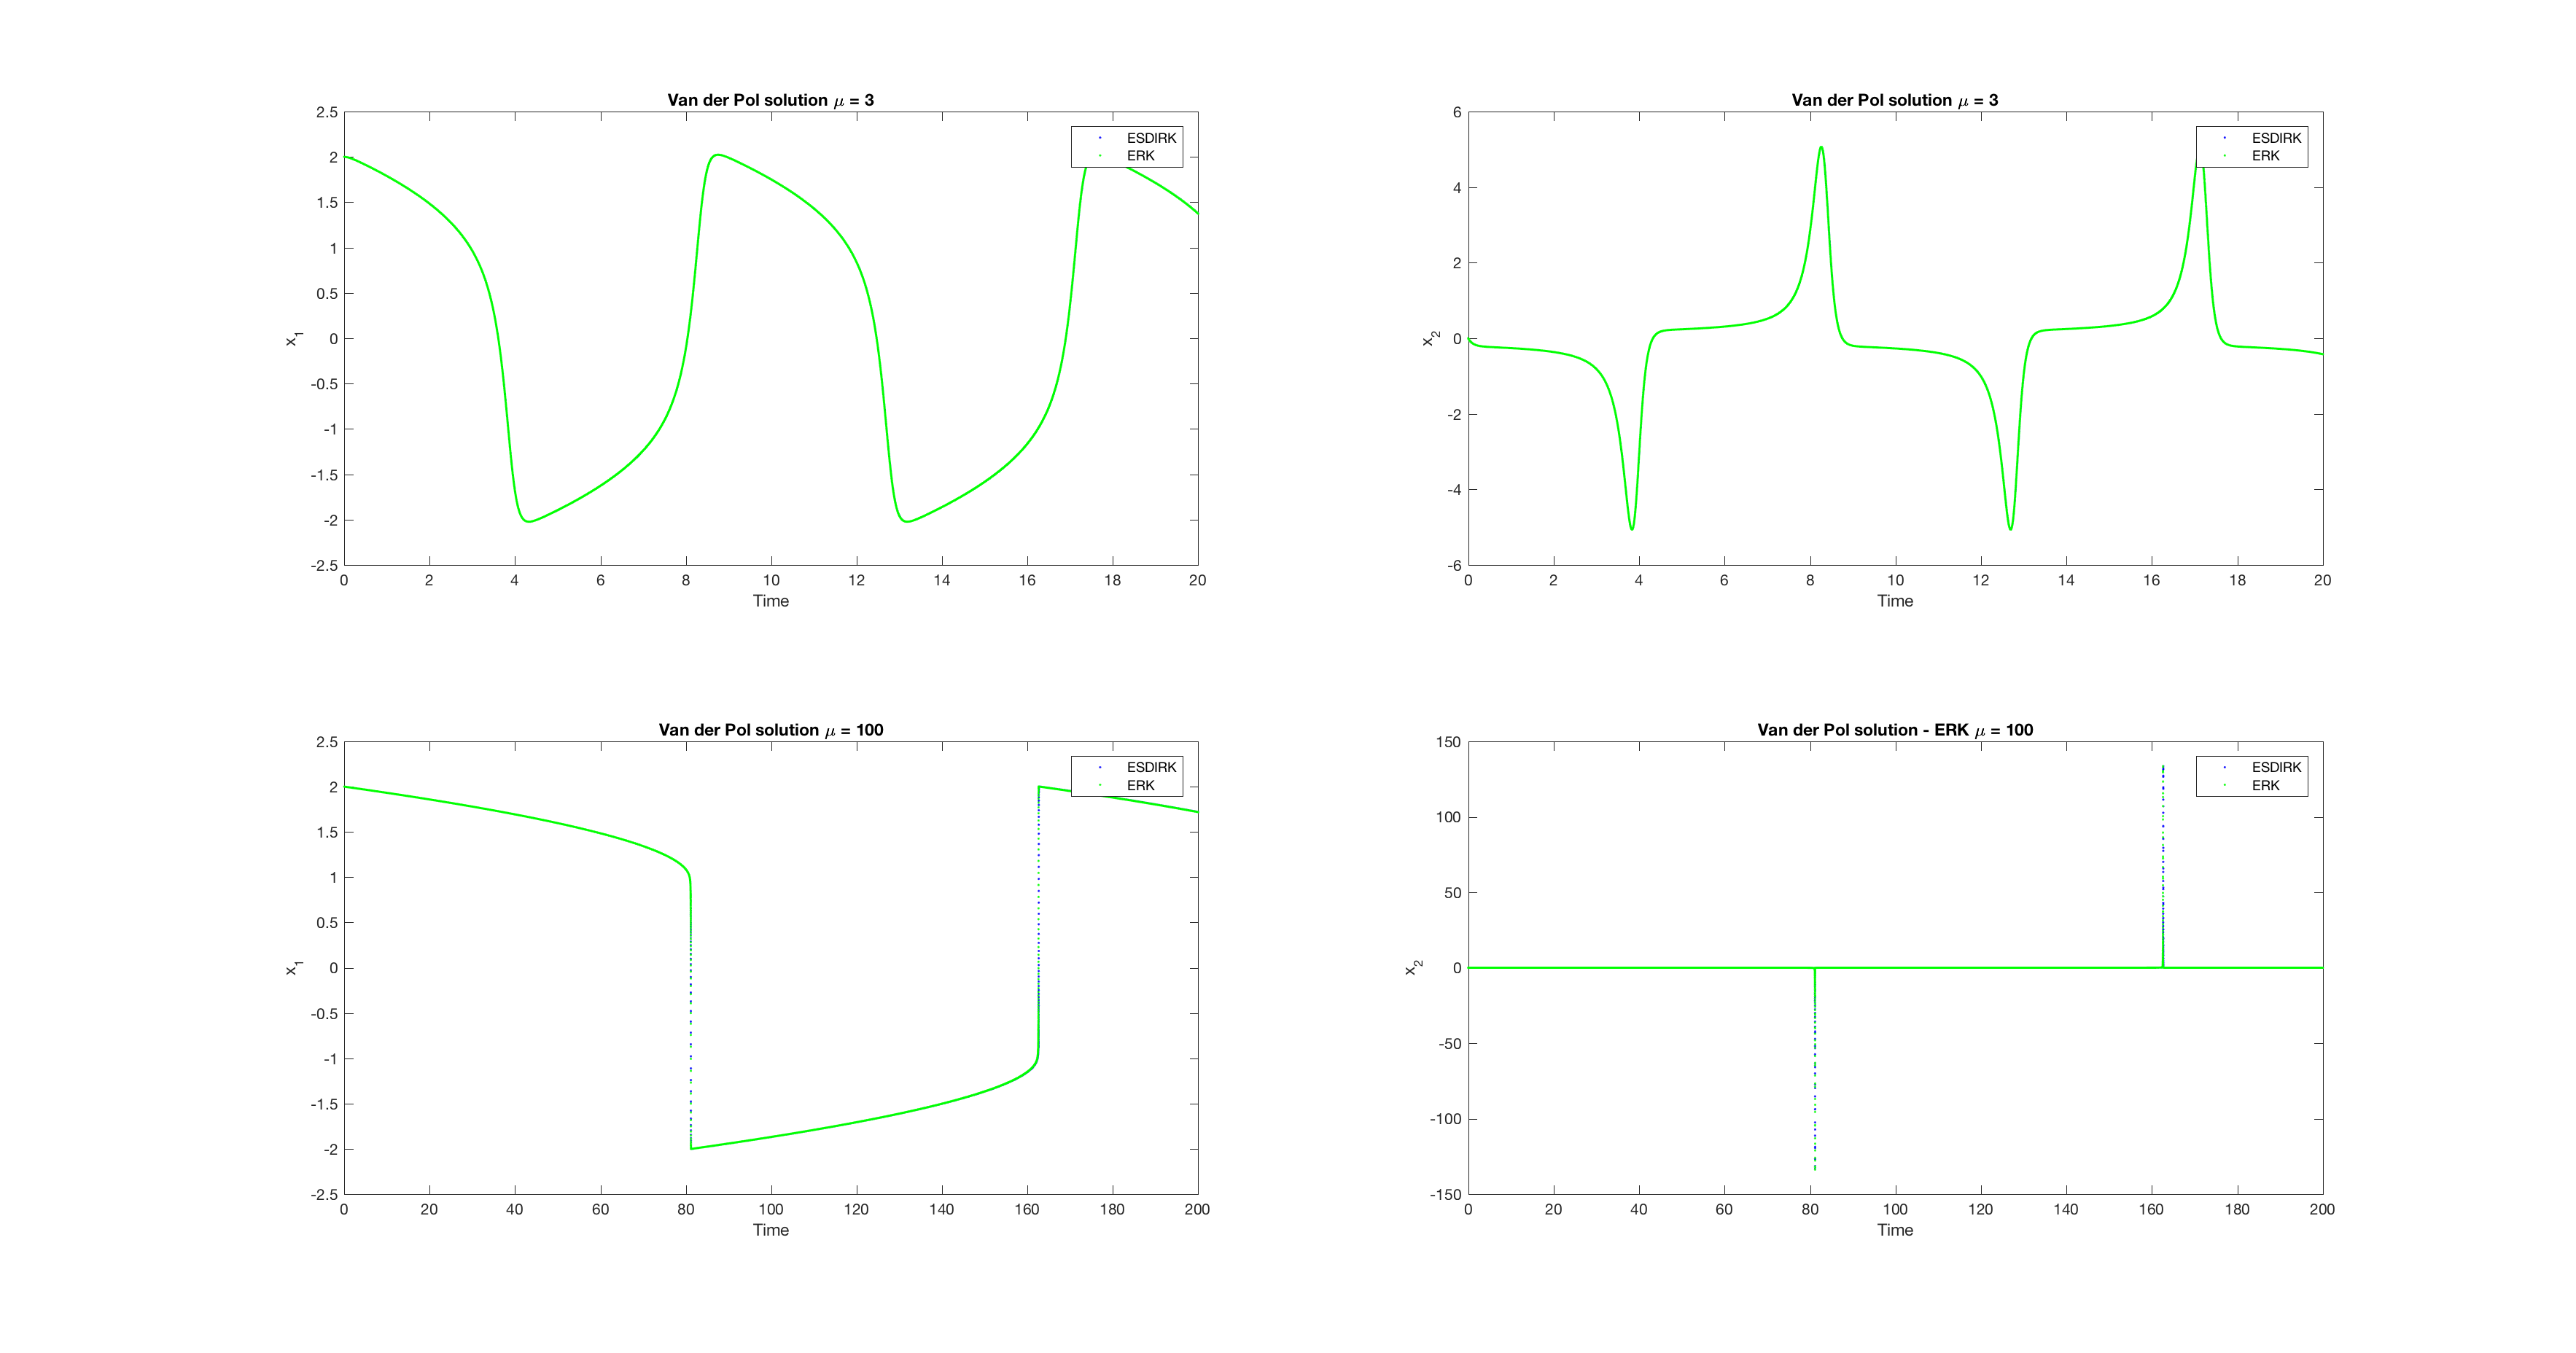
\includegraphics[width=\textwidth]{../Figures/ex5_vanderpol}
    \caption{ESDIRK23 vs our ERK method on the Van der Pol problem with $\mu = 3$ and $\mu = 100$ (stiff)}
    \label{fig:ex5comparison}
\end{figure}

\subsection{Stability region, A and L-stability, practical implications}
%Plot the stability region of the ESDIRK23 method. Is it A-stable? Is
%it L-stable? Discuss the practical implications of the stability region of
%ESDIRK23.
We can rewrite the stability function $R(z)$ as $R(z) = 1 + z b^T (I - z A)^{-1} e = \frac{\text{det}(I - zA + zeb^T)}{\text{det}(I-zA)}$ and using Mathematica or Matlab's Symbolic Toolbox explicitly calculate the numerator and denominator resulting in $R(z) = \frac{z-2z\gamma+1}{(\gamma z - 1)^2} = \frac{1+z(1-2 \gamma)}{(1-\gamma z)^2}$. L-stability is defined as $\lim_{z \to \infty}|R(z)| = 0$, again using Matlab we can verify that is holds or simply applying L'Hospital's rule once on the fraction yielding 0.

\begin{figure}[H]
    \centering
    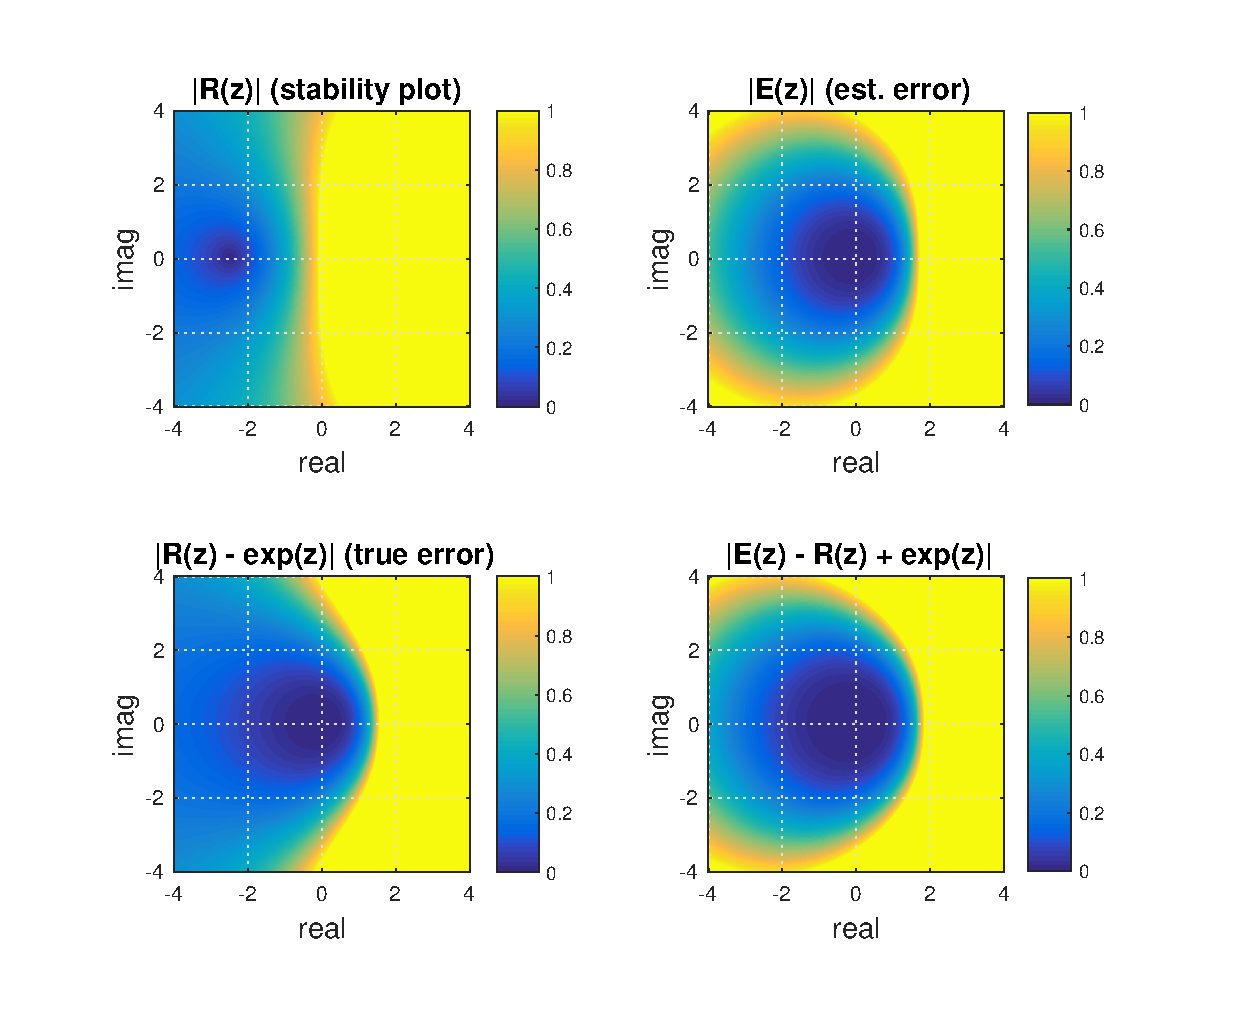
\includegraphics[width=\textwidth]{../Figures/ex5_stability}
    \caption{ESDIRK23 stability summary}
\end{figure}

Since the left half plane of $|R(z)|<1$, we can conclude that the method is A-stable. From the Definition 8.2 in LeVeque we verified that this method is also L-stable (because it is A-stable and the previously mentioned limit is equal to 0). Even though the method is A and L-stable it's not suitable when $\lambda > 1$ because it is unstable as can be seen in the right halfplane of $|R(z)|$. Another thing worth noting is that the explicit Runge-Kutta methods (like question 3) have bounded stability region increasing with the order (hence they can never be A-stable) in contrast to implicit methods like ESDIRK23 or the trapezoidal method that cover the left complex plane.



\subsection{Implementation with variable step size and testing on Van der Pol problem}
% Implement ESDIRK23 with variable step size. Test it on the Van der Pol problem.
As mentioned in the first part of this section the implementation is based on the given ESDIRK code in the lecture files folder. Similarly there is again no need for the $g$ function as discussed before, but the step size control is kept and adapted to use the IVP in terms of $f(t,\mathbf{x})$ and $\mathbf{x}(t)$.

Firstly we step into the "main" loop thar runs until we reach the final time and for all stages calculate the initial point (along with convergence check) and use Newton's iterations (to obtain approximate $X_i$), which keep running only if we haven't converged and we are not diverging as well as not converging too slowly (Jacobian approximation worsens meaning more iterations are needed to coverge), otherwise the iteration is halted. Then we decide based on convergence of the iterations whether to branch into error estimatation, step length controller (consequentialy accepting the step and using PI/Asymptotic controller for hr), perform convergence control for the step size and the Jacobian update strategy (evaluation and LU factorization) or just update the step size based on divergence or the freshness of Jacobian and calculate new LU factorization. In the end if the estimated error is small enough a step is taken.

Matlab code for this implementation is in the appendix.